\secnumbersection{EXPERIMENTACIÓN}

En el presente capítulo se realiza se describe la experimentación realizada durante el desarrollo de la memoria, es decir, se lleva a cabo la cuantificación del modelo matemático, se describe la calibración de los sensores utilizados y se detallan los resultados en cada uno de los 5 ambientes descritos en el capítulo anterior.

\subsection{CUANTIFICACIÓN DEL MODELO MATEMÁTICO}

En el capítulo anterior se desarrolló el modelo matemático que define la odometría del robot a partir de los encoders de las ruedas, por lo que en esta sección se cuantificará dicho modelo para obtener las fórmulas correspondientes que se utilizarán en el desarrollo de la memoria.
El modelo matemático viene dado por las Ecuaciones \ref{ecuacion_1}, \ref{ecuacion_2} y \ref{ecuacion_3}, luego para obtener la relación entre los encoders y la distancia recorrida se realizaron 10 test, en dónde se analizó la cantidad de ticks obtenidos en un metro y en medio giro por cada encoder, los cuales se pueden observar en la Tabla \ref{tab:encoders_data}.

\begin{table}[H]
\centering
\begin{tabular}{@{}ccccc@{}}
\toprule
                                  & \textbf{\begin{tabular}[c]{@{}c@{}}Ticks derecho\\ en un metro\end{tabular}} & \textbf{\begin{tabular}[c]{@{}c@{}}Ticks izquierdo\\ en un metro\end{tabular}} & \textbf{\begin{tabular}[c]{@{}c@{}}Ticks derecho\\ en giro de 180°\end{tabular}} & \textbf{\begin{tabular}[c]{@{}c@{}}Ticks izquierdo\\ en giro de 180°\end{tabular}} \\ \midrule
\multicolumn{1}{|c|}{\textbf{1}}  & \multicolumn{1}{c|}{11.154}                                                  & \multicolumn{1}{c|}{1.140}                                                     & \multicolumn{1}{c|}{3.574}                                                       & \multicolumn{1}{c|}{452}                                                           \\ \midrule
\multicolumn{1}{|c|}{\textbf{2}}  & \multicolumn{1}{c|}{10.868}                                                  & \multicolumn{1}{c|}{1.134}                                                     & \multicolumn{1}{c|}{3.653}                                                       & \multicolumn{1}{c|}{444}                                                           \\ \midrule
\multicolumn{1}{|c|}{\textbf{3}}  & \multicolumn{1}{c|}{9.931}                                                   & \multicolumn{1}{c|}{1.146}                                                     & \multicolumn{1}{c|}{3.307}                                                       & \multicolumn{1}{c|}{384}                                                           \\ \midrule
\multicolumn{1}{|c|}{\textbf{4}}  & \multicolumn{1}{c|}{9.935}                                                   & \multicolumn{1}{c|}{1.132}                                                     & \multicolumn{1}{c|}{3.057}                                                       & \multicolumn{1}{c|}{378}                                                           \\ \midrule
\multicolumn{1}{|c|}{\textbf{5}}  & \multicolumn{1}{c|}{9.581}                                                   & \multicolumn{1}{c|}{1.142}                                                     & \multicolumn{1}{c|}{3.074}                                                       & \multicolumn{1}{c|}{382}                                                           \\ \midrule
\multicolumn{1}{|c|}{\textbf{6}}  & \multicolumn{1}{c|}{9.944}                                                   & \multicolumn{1}{c|}{1.123}                                                     & \multicolumn{1}{c|}{3.303}                                                       & \multicolumn{1}{c|}{351}                                                           \\ \midrule
\multicolumn{1}{|c|}{\textbf{7}}  & \multicolumn{1}{c|}{9.000}                                                   & \multicolumn{1}{c|}{1.138}                                                     & \multicolumn{1}{c|}{3.233}                                                       & \multicolumn{1}{c|}{374}                                                           \\ \midrule
\multicolumn{1}{|c|}{\textbf{8}}  & \multicolumn{1}{c|}{10.265}                                                  & \multicolumn{1}{c|}{1.130}                                                     & \multicolumn{1}{c|}{3.315}                                                       & \multicolumn{1}{c|}{344}                                                           \\ \midrule
\multicolumn{1}{|c|}{\textbf{9}}  & \multicolumn{1}{c|}{9.985}                                                   & \multicolumn{1}{c|}{1.121}                                                     & \multicolumn{1}{c|}{3.148}                                                       & \multicolumn{1}{c|}{379}                                                           \\ \midrule
\multicolumn{1}{|c|}{\textbf{10}} & \multicolumn{1}{c|}{9.521}                                                   & \multicolumn{1}{c|}{1.111}                                                     & \multicolumn{1}{c|}{3.112}                                                       & \multicolumn{1}{c|}{367}                                                           \\ \midrule
\textbf{$\bar{x}$} & \textbf{10.008}                                                              & \textbf{1.132}                                                                 & \textbf{3.278}                                                                   & \textbf{386}                                                                       \\ \bottomrule
\end{tabular}
\caption{Valores de los encoders en un metro y medio giro}
\label{tab:encoders_data}
\end{table}

Con los datos obtenidos, se puede observar que en promedio en un metro el encoder derecho cuenta 10.008 ticks y el encoder izquierdo 1.132 ticks. Luego dichos datos se reemplazan en las siguientes fórmulas:
\begin{equation}
    D_i = 2 \cdot \pi \cdot R \cdot \frac{\delta Ticks_i}{\bar{x_i}}
    \label{eq_distance}
\end{equation}

La Fórmula \ref{eq_distance} entrega la distancia recorrida por cada rueda según los ticks correspondientes, es decir, cada rueda corresponde a:
\begin{equation}
    D_{derecha} = 2 \cdot \pi \cdot 0.2 \cdot \frac{\delta Ticks}{10.008}
    \label{eq_distance}
\end{equation}
\begin{equation}
    D_{izquierda} = 2 \cdot \pi \cdot 0.2 \cdot \frac{\delta Ticks}{1.132}
    \label{eq_distance}
\end{equation}

Con estos datos el algoritmo, apoyado con la información del LIDAR puede calcular la odometría, es decir, la posición del robot durante la experimentación.

\subsection{CALIBRACIÓN DE SENSORES}

En la siguiente sección se detallan las diversas calibraciones y resultados de la calibración realizada a los sensores, tales como a la cámara, al sensor IMU y al control utilizado durante la experimentación.

\subsubsection{CALIBRACIÓN DE LA CÁMARA}
Uno de los elementos esenciales a la hora de realizar la memoria es la correcta utilización y por ende, calibración de la cámara de profundidad. Para ello se descargó una plantilla de un tablero de ajedrez cuyas dimensiones de cada cuadrado son de 2.317 centímetros.

\begin{figure}[H]
    \centering
    \begin{subfigure}[b]{0.45\textwidth}
    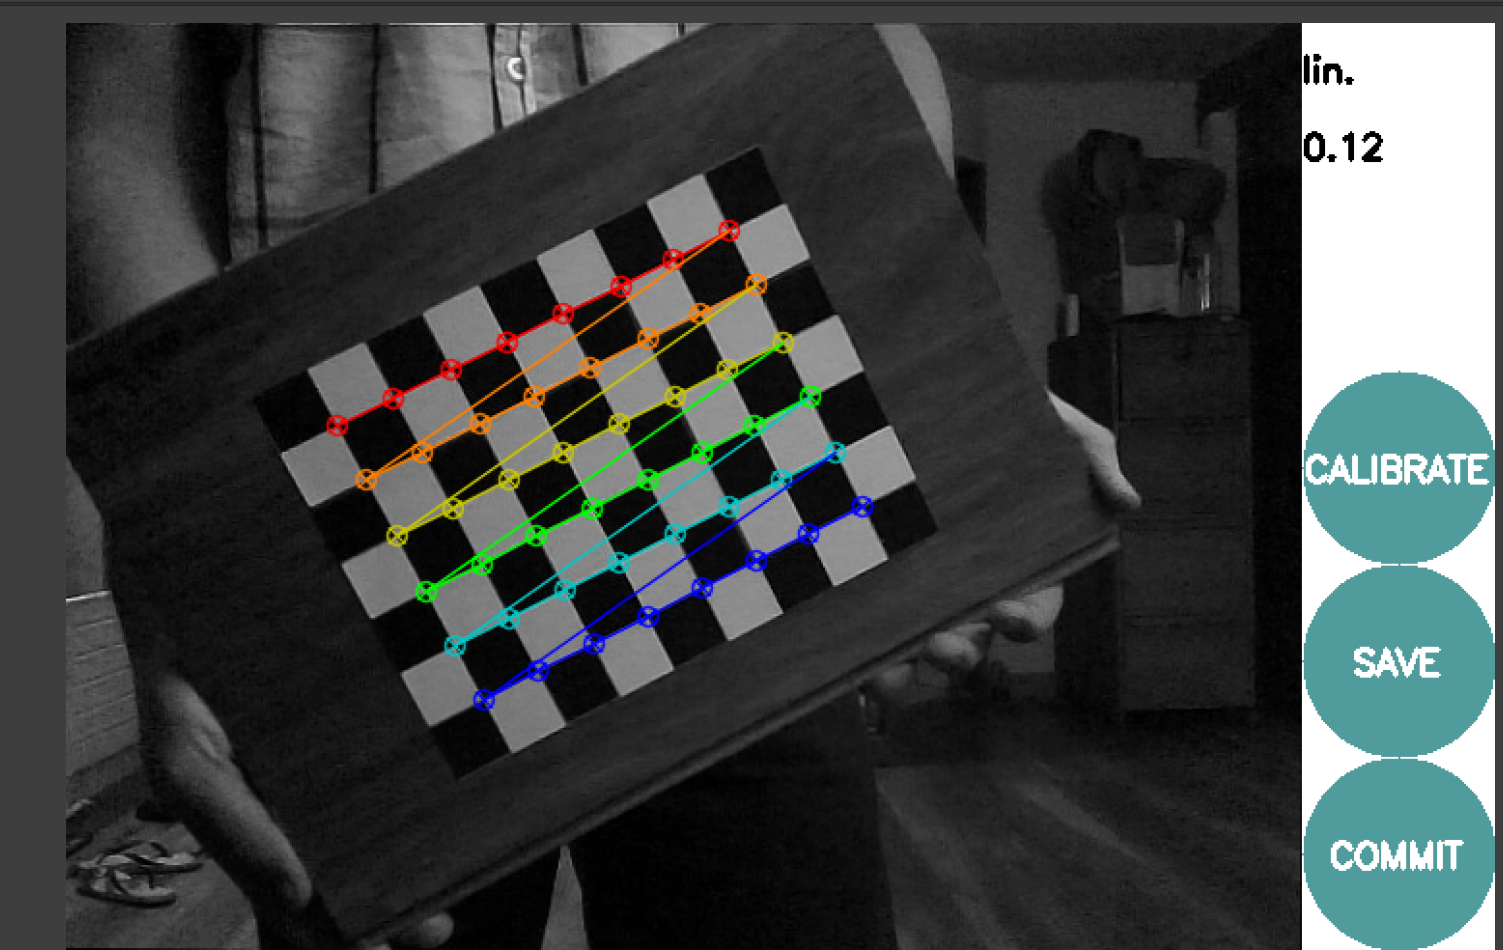
\includegraphics[width=5.5cm, height=5.5cm]{figures/05experimentacion/calibracion_1.png}
    \caption{Obtención de puntos}
    \label{fig:ambiente_1_1}
    \end{subfigure}
    \hspace{10mm}
    \begin{subfigure}[b]{0.45\textwidth}
    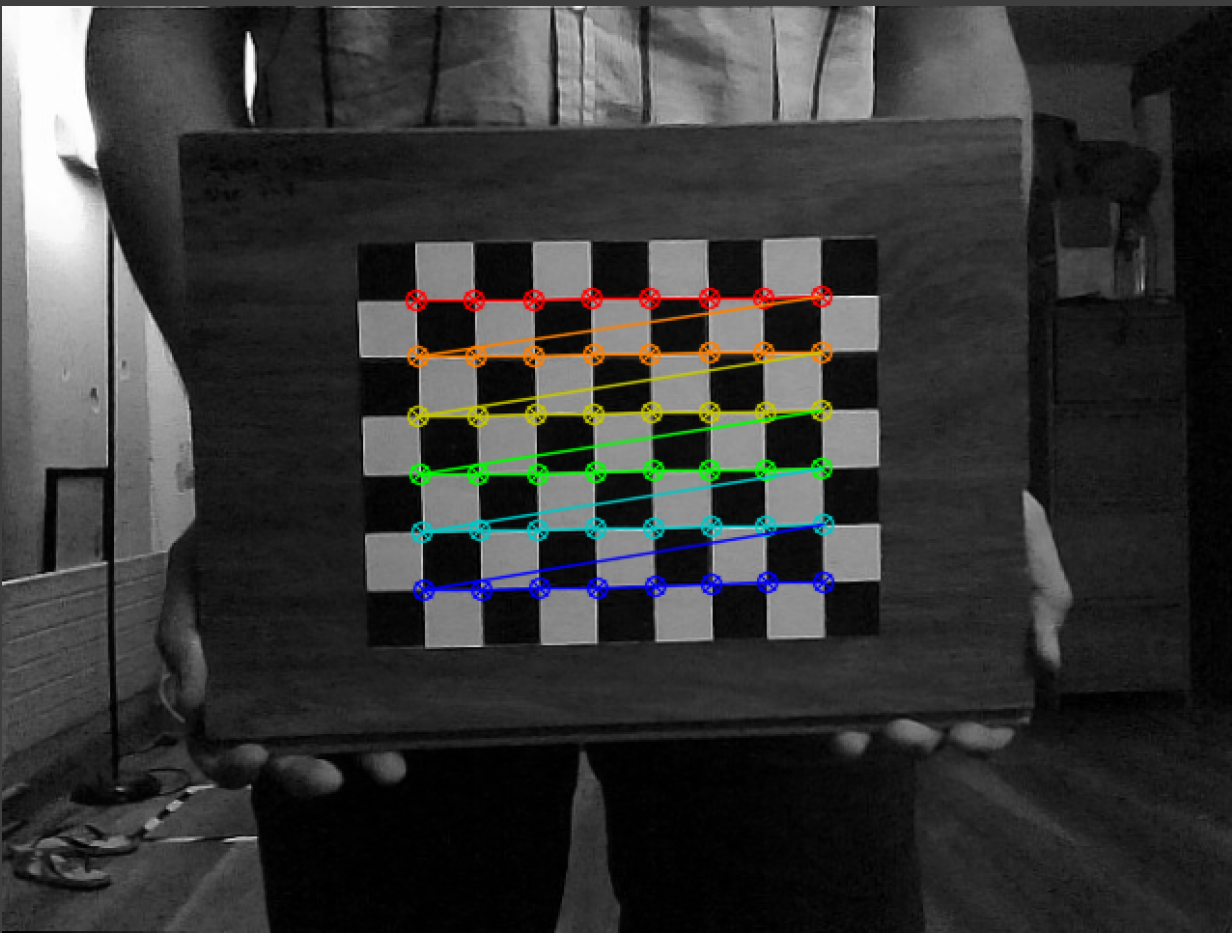
\includegraphics[width=5.5cm, height=5.5cm]{figures/05experimentacion/calibracion_2.png}
    \caption{Cámara calibrada}
    \label{fig:ambiente_1_2}
    \end{subfigure}
    \caption{Proceso de calibración de la cámara}
    Fuente: Fabricación propia
    \label{fig:ambiente_1}
\end{figure} 

Con esta información y el paquete camera\_calibration, se procede a realizar la calibración de la cámara obteniendo los siguientes resultados:
\begin{verbatim}
image_width: 640
image_height: 480
camera_name: narrow_stereo
camera_matrix:
  rows: 3
  cols: 3
  data: [963.23519,   0.     , 380.06762,
           0.     , 963.76291, 277.39557,
           0.     ,   0.     ,   1.     ]
distortion_model: plumb_bob
distortion_coefficients:
  rows: 1
  cols: 5
  data: [0.119060, -0.442568, 0.012033, -0.010606, 0.000000]
rectification_matrix:
  rows: 3
  cols: 3
  data: [1., 0., 0.,
         0., 1., 0.,
         0., 0., 1.]
projection_matrix:
  rows: 3
  cols: 4
  data: [976.87628,   0.     , 376.06458,   0.     ,
           0.     , 974.24756, 280.33573,   0.     ,
           0.     ,   0.     ,   1.     ,   0.     ]
\end{verbatim}

\subsubsection{CALIBRACIÓN DEL IMU}
La Unidad de Medida Inercial utilizada durante la memoria requería ser calibrada siguiendo un par de procesos físicos los cuales se centran en movimientos circulares, movimientos verticales y movimientos rotacionales. Sin embargo, además de dicha calibración era requerido desempaquetar los datos provenientes del sensor, los cuales provienen en formato binario, para ello se realizó un filtro a la cabecera y se desempaquetó los datos según corresponda utilizando el siguiente código:
\begin{verbatim}
    def euler_to_quaternion(roll, pitch, yaw):
        rot = Rotation.from_euler('xyz', [yaw, pitch, roll], degrees=True)
        q = rot.as_quat()
        q = np.round(q, 3)
        return q[::-1]
        
    if data[0] == 0x61 and len(data) == 20:
        # Acceleration data
        acc = np.array(struct.unpack('<hhh', data[1:7]))/32768.0*16.0*9.8
        acc = np.round(acc, 3)

        # Angular velocity data
        gyro = np.array(struct.unpack('<hhh', data[7:13]))/32768.0*2000.0
        gyro = np.round(gyro, 3)
            
        # Angle data
        angle = np.array(struct.unpack('<hhh', data[13:19]))/32768.0*180.0
        angle = np.round(angle, 3)
        q = euler_to_quaternion(angle[0], angle[1], angle[2])
\end{verbatim}

Cabe destacar que las multiplicaciones pertinentes se realizaron siguiendo las instrucciones del proveedor del sensor. El código en detalle se puede observar en la sección de Anexos.

\subsubsection{CALIBRACIÓN DEL CONTROL}
Con respecto al control bluetooth utilizado para desarrollar la memoria, era necesario realizar la calibración para ser utilizado en conjunto del framework ROS por lo que se realizó la calibración con el paquete ds4\_joystick. Luego de la calibración se procedió a desempaquetar los datos utilizando los mensajes del tipo Joy utilizando el siguiente código:
\begin{verbatim}
    def chatter_callback(mensaje):
        joystick_izquierdo = (
            round(mensaje.axes[0], 3), 
            round(mensaje.axes[1], 3))
        joystick_derecho = (
            round(mensaje.axes[2], 3), 
            round(mensaje.axes[5], 3))
        botones = (
            mensaje.buttons[1], 
            mensaje.buttons[2], 
            mensaje.buttons[3], 
            mensaje.buttons[0]) 
\end{verbatim}
ROS provee de herramientas para analizar la utilización de controles externos a través de los mensajes del tipo Joy, de esta manera se pueden analizar el estado de los joysticks, cruces y botones del control utilizado. El código en detalles se puede observar en la sección de Anexos.

\subsection{RESULTADOS Y ANÁLISIS}
A continuación se presentan los resultados y un análisis previo por cada ambiente descrito en el capítulo anterior. El análisis se realizará en base a las métricas descritas y la comparación con otros 2 algoritmos SLAM:
\begin{itemize}
    \item \textbf{OctoMap Library:} Librería que implementa un algoritmo de SLAM tridimensional donde la construcción mapa se realiza mediante octree y diseñada para suplir los siguientes requerimientos: Un modelado tridimensional completo, con capacidad de actualizar los datos en tiempo real, flexible sobre la dimensión física del mapa y finalmente un algoritmo que compacta el mapa generado para ocupar la menor cantidad de memoria. Es decir, es una paquete centrado en la construcción del mapa tridimensional pero no en la localización o navegación.
    \item \textbf{Hector Mapping:} Paquete que implementa un algoritmo SLAM en donde no se requiere información sobre la odometría del robot, por lo que solo utiliza la información del LIDAR para ubicar el robot en el mapa. Es un algoritmo de mapeo bidimensional por lo que solo genera un mapa 2D del ambiente. El algoritmo se centra en la localización y mapeo del ambiente, siendo un punto bastante débil la navegación del robot.
\end{itemize}

De esta manera el algoritmo propuesto se compara directamente con el desempeño de un algoritmo SLAM y un algoritmo SLAM 3D, dado que además de generar un mapa tridimensional, el algoritmo genera un mapa bidimensional del espacio y permite la navegación sobre este. Una vez dispuestas las métricas por cada algoritmo se procederá a realizar un análisis comparativo de los 3 algoritmos a través del comportamiento de en cada ambiente.

\subsubsection{RESULTADOS EN EL AMBIENTE NÚMERO 1}

En la Figura \ref{fig:ambiente_1} se observa el proceso de mapeo del ambiente 1. El mapeo se inicia en la posición inicial, de esta manera queda identificada la posición (0,0) en el mapa como el inicio, por otro lado, en colores se puede observar el mapa tridimensional, mientras que en gris el mapa bidimensional, a su vez se destaca en color rojo los datos del lidar con los cuales se realiza la corrección de los datos obtenidos por la cámara de profundidad. 

\begin{figure}[H]
    \centering
    \begin{subfigure}[b]{0.30\textwidth}
    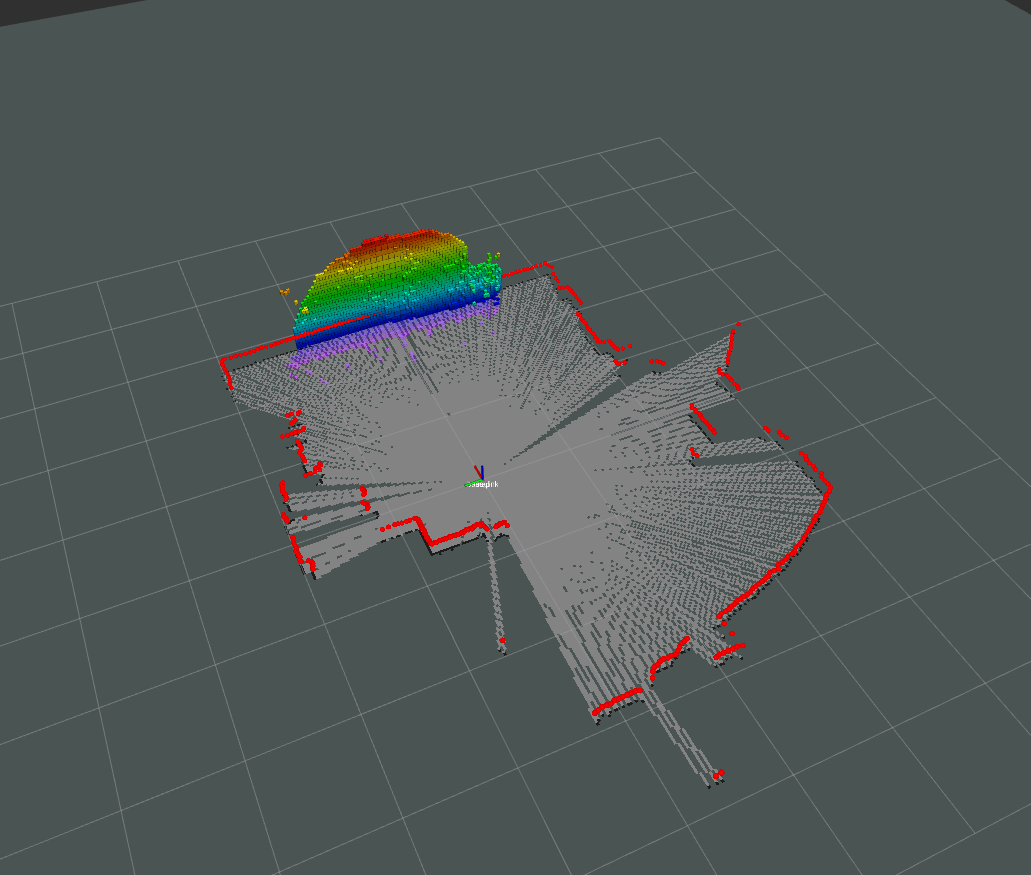
\includegraphics[width=\textwidth, height=\textwidth]{figures/05experimentacion/ambiente_1/r00_01.png}
    \caption{Inicio del mapeo}
    \label{fig:ambiente_1_1}
    \end{subfigure}
    \begin{subfigure}[b]{0.30\textwidth}
    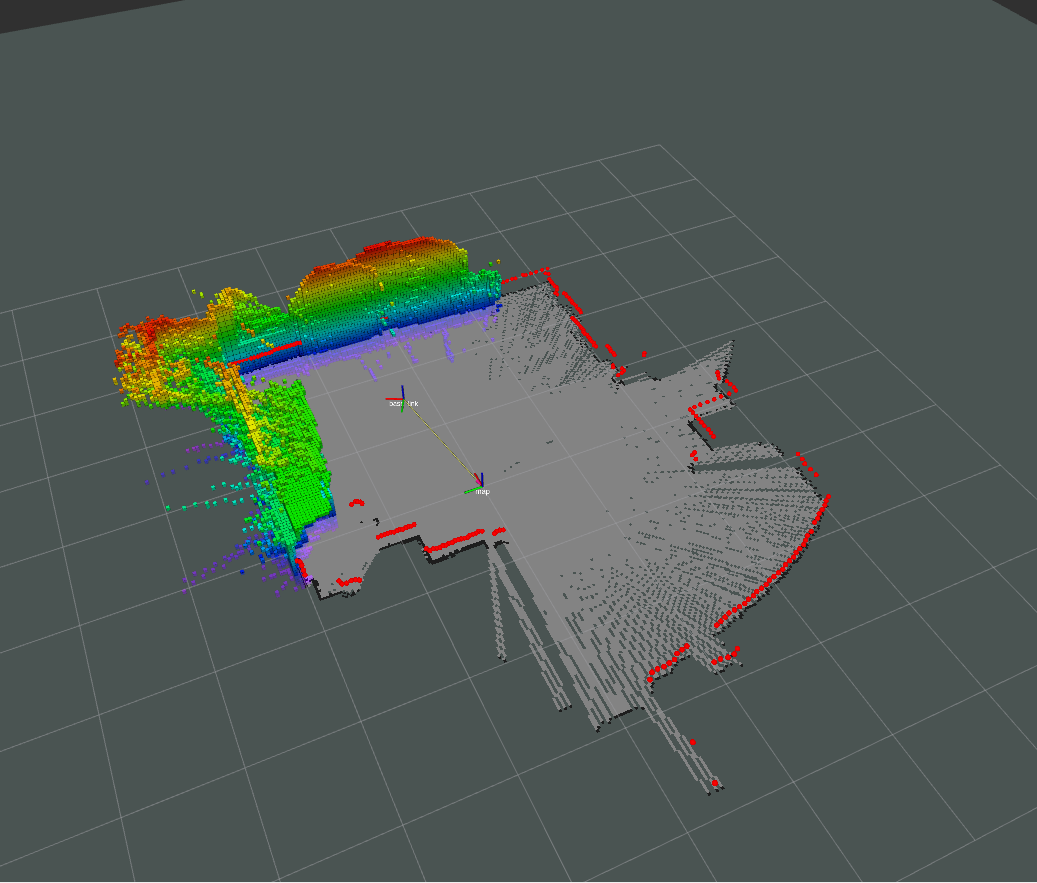
\includegraphics[width=\textwidth, height=\textwidth]{figures/05experimentacion/ambiente_1/r00_02.png}
    \caption{En proceso del mapeo}
    \label{fig:ambiente_1_2}
    \end{subfigure}
    \begin{subfigure}[b]{0.30\textwidth}
    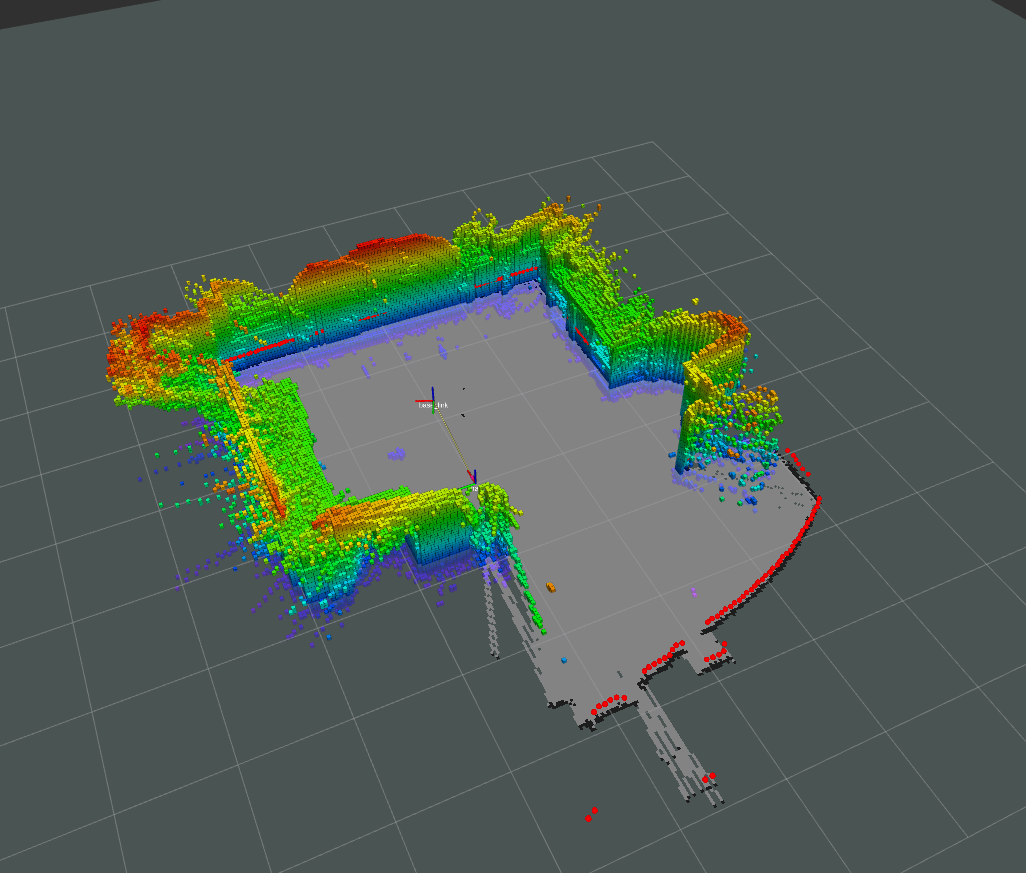
\includegraphics[width=\textwidth, height=\textwidth]{figures/05experimentacion/ambiente_1/r00_03.png}
    \caption{Ambiente mapeado}
    \label{fig:ambiente_1_3}
    \end{subfigure}
    \caption{Proceso de mapeo del ambiente 1}
    Fuente: Fabricación propia
    \label{fig:ambiente_1}
\end{figure} 

A continuación, en la Tabla \ref{tab:resultados_ambiente_1} se identifican el valor de las métricas obtenidas durante la experimentación en el ambiente 1. Se puede destacar como el algoritmo propuesto en las métricas asociadas al mapeo tiene un mejor desempeño que el algoritmo tridimensional OctoMap y que a su vez, el desempeño en las tareas de navegación y localización están a la par con el algoritmo bidimensional Hector. 


\begin{table}[H]
\centering
\begin{tabular}{@{}lccc@{}}
\toprule
\multicolumn{1}{|c|}{\textbf{Métrica}} &
  \multicolumn{1}{c|}{\textbf{OctoMap Library}} &
  \multicolumn{1}{c|}{\textbf{Hector Mapping}} &
  \multicolumn{1}{c|}{\textbf{Algoritmo Propuesto}} \\ \midrule
\multicolumn{1}{|l|}{\textbf{Tiempo en generar el mapa}}    & \multicolumn{1}{c|}{17,782} & \multicolumn{1}{c|}{5,542} & \multicolumn{1}{c|}{12,641} \\ \midrule
\multicolumn{1}{|l|}{\textbf{Precisión del mapa generado}}  & \multicolumn{1}{c|}{97,27\%} & \multicolumn{1}{c|}{92,21\%} & \multicolumn{1}{c|}{96,27\%} \\ \midrule
\multicolumn{1}{|l|}{\textbf{Ruta planificada}}             & \multicolumn{1}{c|}{4,486} & \multicolumn{1}{c|}{3,149} & \multicolumn{1}{c|}{3,204} \\ \midrule
\multicolumn{1}{|l|}{\textbf{Precisión de la ruta}}         & \multicolumn{1}{c|}{90,71\%} & \multicolumn{1}{c|}{98,23\%} & \multicolumn{1}{c|}{98,01\%} \\ \midrule
\multicolumn{1}{|l|}{\textbf{Tiempo en completar la ruta}}  & \multicolumn{1}{c|}{8,992} & \multicolumn{1}{c|}{7,103} & \multicolumn{1}{c|}{7,479} \\ \midrule
\multicolumn{1}{|l|}{\textbf{Tiempo de localización}}       & \multicolumn{1}{c|}{2,751} & \multicolumn{1}{c|}{1,924} & \multicolumn{1}{c|}{1,972} \\ \midrule
\multicolumn{1}{|l|}{\textbf{Precisión de la localización}} & \multicolumn{1}{c|}{80,74\%} & \multicolumn{1}{c|}{95,71\%} & \multicolumn{1}{c|}{97,01\%} \\ \midrule
\multicolumn{1}{|l|}{\textbf{Adaptación}}                   & \multicolumn{1}{c|}{True} & \multicolumn{1}{c|}{True} & \multicolumn{1}{c|}{True} \\ \midrule
\multicolumn{1}{|l|}{\textbf{Consumo de memoria}}           & \multicolumn{1}{c|}{1.749} & \multicolumn{1}{c|}{1.024} & \multicolumn{1}{c|}{1.988} \\ \midrule
\multicolumn{1}{|l|}{\textbf{Tamaño del archivo}}           & \multicolumn{1}{c|}{0,8916} & \multicolumn{1}{c|}{0,013} & \multicolumn{1}{c|}{0,9196} \\ \bottomrule
\end{tabular}
\caption{Resultados en Ambiente 1}
\label{tab:resultados_ambiente_1}
\end{table}

Por otro lado, las trayectorias realizadas por los algoritmos se puede observar en la Figura \ref{fig:tray_01}, en donde se observa un comportamiento similar entre el algoritmo propuesto y el algoritmo Hector, sin embargo, se nota una leve diferencia en la trayectoria realizada con el algoritmo OctoMap, lo que conlleva a una ruta planificada más larga y un mayor tiempo para completar la ruta.

\begin{figure}[H]
    \centering
    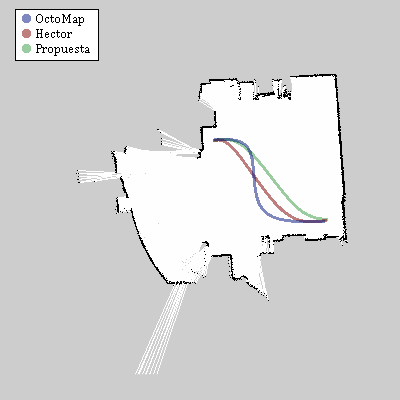
\includegraphics[width=0.5\textwidth]{figures/05experimentacion/r00.png}
    \caption{ Comparación de las trayectorias realizadas por los algoritmos en el ambiente 1} 
    \label{fig:tray_01}
    Fuente: Fabricación propia
\end{figure}

\subsubsection{RESULTADOS EN EL AMBIENTE NÚMERO 2}

En la Figura \ref{fig:ambiente_2} se observa el proceso de mapeo del ambiente 2. Al igual que en el ambiente 1, el mapeo se inicia en la posición inicial por lo que en dicha posición queda iniciado el mapa. Además de las paredes externas observadas en la Figura, se pueden identificar el obstáculo 1 y el obstáculo 2 al centro del ambiente mapeado. 
\begin{figure}[H]
    \centering
    \begin{subfigure}[b]{0.30\textwidth}
    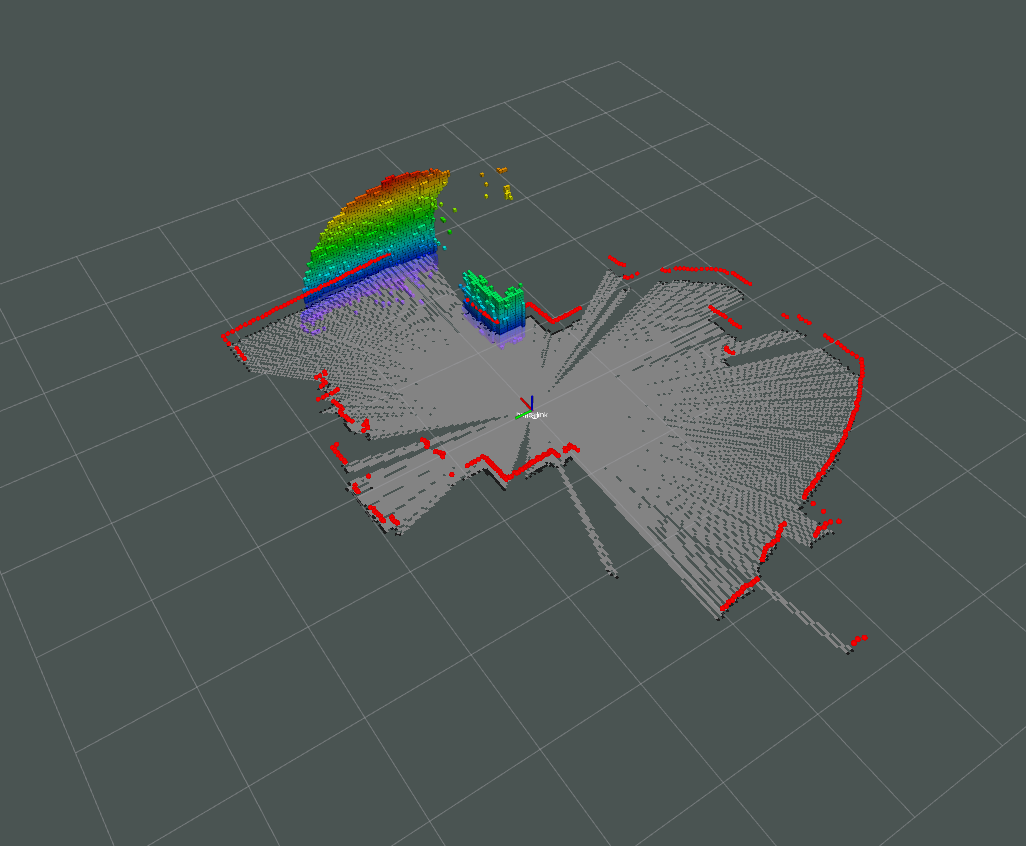
\includegraphics[width=\textwidth, height=\textwidth]{figures/05experimentacion/ambiente_2/r01_01.png}
    \caption{Inicio del mapeo}
    \label{fig:ambiente_2_1}
    \end{subfigure}
    \begin{subfigure}[b]{0.30\textwidth}
    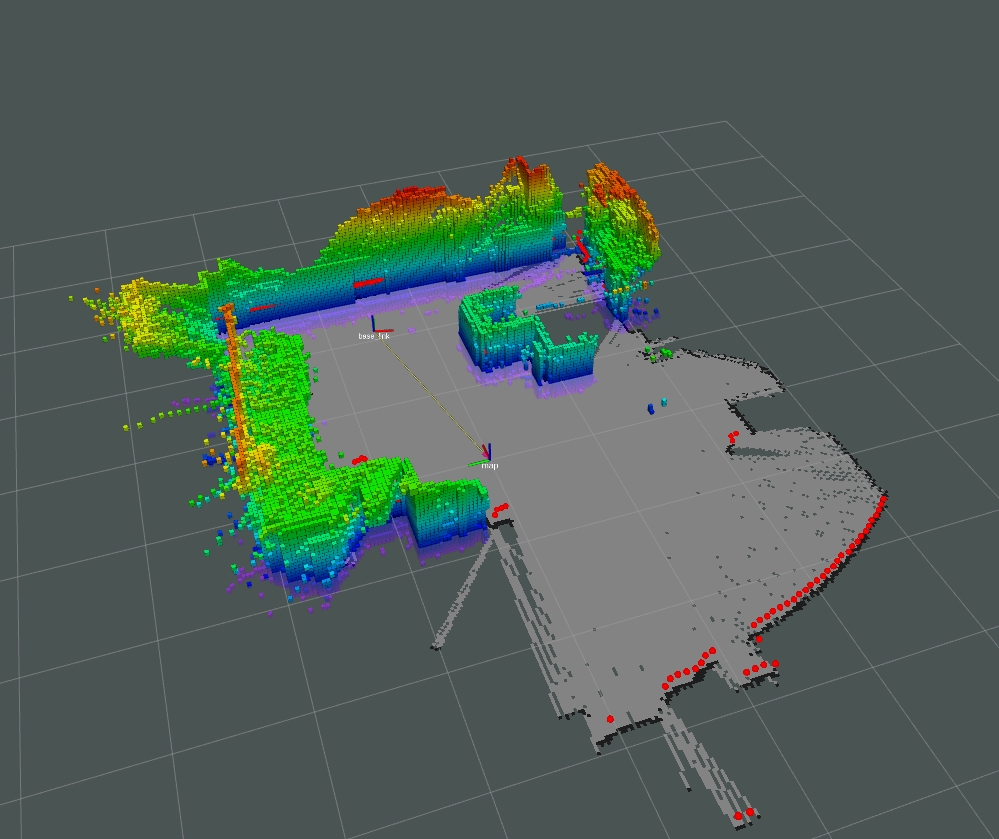
\includegraphics[width=\textwidth, height=\textwidth]{figures/05experimentacion/ambiente_2/r01_02.png}
    \caption{En proceso del mapeo}
    \label{fig:ambiente_2_2}
    \end{subfigure}
    \begin{subfigure}[b]{0.30\textwidth}
    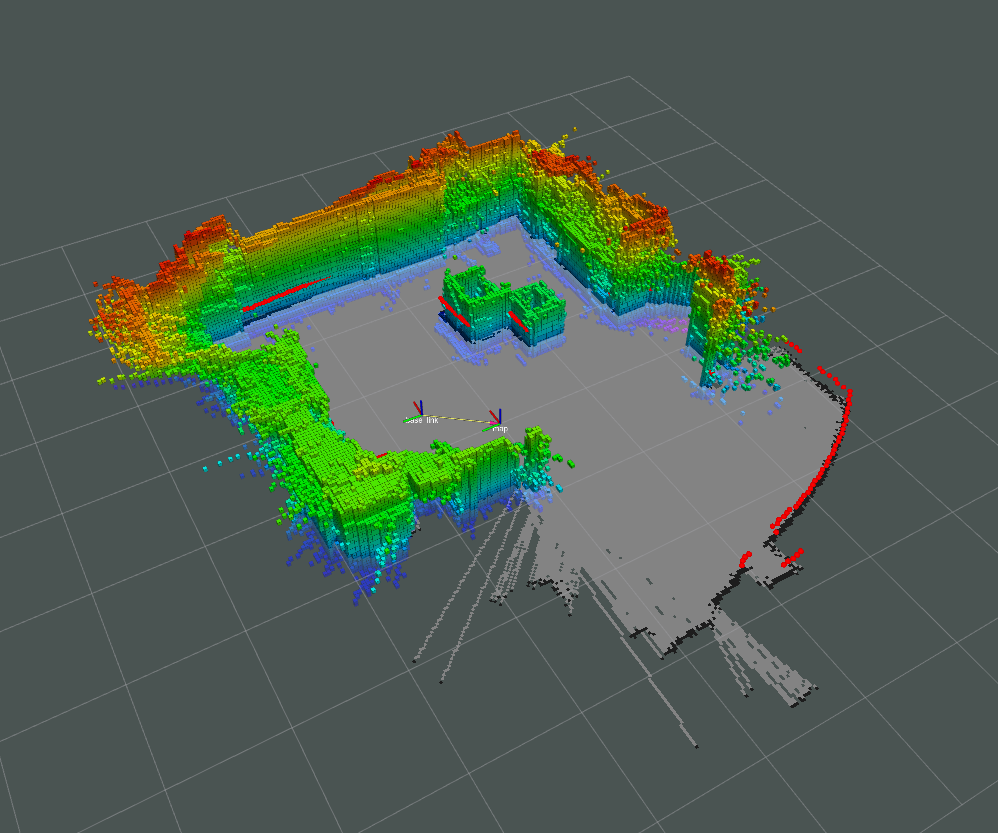
\includegraphics[width=\textwidth, height=\textwidth]{figures/05experimentacion/ambiente_2/r01_03.png}
    \caption{Ambiente mapeado}
    \label{fig:ambiente_2_3}
    \end{subfigure}
    \caption{Proceso de mapeo del ambiente 2}
    Fuente: Fabricación propia
    \label{fig:ambiente_2}
\end{figure} 

En la Tabla \ref{tab:resultados_ambiente_2} se pueden encontrar el comportamiento de las métricas por los 3 algoritmos evaluados en el ambiente 2. Se observa como los algoritmos SLAM 3D (OctoMap Library y el algoritmo propuesto) les toma el doble de tiempo en generar el mapa en comparación con el algoritmo Hector. También se observa que el comportamiento general del algoritmo propuesto en las tareas asociadas al mapeo se sigue manteniendo favorable en comparación al algoritmo OctoMap y en las tareas asociadas a la navegación y localización se comporta de manera similar con el algoritmo Hector.

\begin{table}[H]
\centering
\begin{tabular}{@{}lccc@{}}
\toprule
\multicolumn{1}{|c|}{\textbf{Métrica}} &
  \multicolumn{1}{c|}{\textbf{OctoMap Library}} &
  \multicolumn{1}{c|}{\textbf{Hector Mapping}} &
  \multicolumn{1}{c|}{\textbf{Algoritmo Propuesto}} \\ \midrule
\multicolumn{1}{|l|}{\textbf{Tiempo en generar el mapa}}    & \multicolumn{1}{c|}{21,121} & \multicolumn{1}{c|}{7,452} & \multicolumn{1}{c|}{15,947} \\ \midrule
\multicolumn{1}{|l|}{\textbf{Precisión del mapa generado}}  & \multicolumn{1}{c|}{97,47\%} & \multicolumn{1}{c|}{90,63\%} & \multicolumn{1}{c|}{91,75\%} \\ \midrule
\multicolumn{1}{|l|}{\textbf{Ruta planificada}}             & \multicolumn{1}{c|}{5,678} & \multicolumn{1}{c|}{4,196} & \multicolumn{1}{c|}{4,053} \\ \midrule
\multicolumn{1}{|l|}{\textbf{Precisión de la ruta}}         & \multicolumn{1}{c|}{89,57\%} & \multicolumn{1}{c|}{95,74\%} & \multicolumn{1}{c|}{93,17\%} \\ \midrule
\multicolumn{1}{|l|}{\textbf{Tiempo en completar la ruta}}  & \multicolumn{1}{c|}{11,024} & \multicolumn{1}{c|}{8,478} & \multicolumn{1}{c|}{8,549} \\ \midrule
\multicolumn{1}{|l|}{\textbf{Tiempo de localización}}       & \multicolumn{1}{c|}{2,541} & \multicolumn{1}{c|}{1,376} & \multicolumn{1}{c|}{1,126} \\ \midrule
\multicolumn{1}{|l|}{\textbf{Precisión de la localización}} & \multicolumn{1}{c|}{83,17\%} & \multicolumn{1}{c|}{96,24\%} & \multicolumn{1}{c|}{98,11\%} \\ \midrule
\multicolumn{1}{|l|}{\textbf{Adaptación}}                   & \multicolumn{1}{c|}{True} & \multicolumn{1}{c|}{True} & \multicolumn{1}{c|}{True} \\ \midrule
\multicolumn{1}{|l|}{\textbf{Consumo de memoria}}           & \multicolumn{1}{c|}{1.801} & \multicolumn{1}{c|}{1.102} & \multicolumn{1}{c|}{2.133} \\ \midrule
\multicolumn{1}{|l|}{\textbf{Tamaño del archivo}}           & \multicolumn{1}{c|}{0,871} & \multicolumn{1}{c|}{0,023} & \multicolumn{1}{c|}{0,963} \\ \bottomrule
\end{tabular}
\caption{Resultados en Ambiente 2}
\label{tab:resultados_ambiente_2}
\end{table}

En la Figura \ref{fig:tray_02} se pueden identificar las trayectorias de los 3 algoritmos durante la experimentación en el ambiente 2. Se observa claramente un comportamiento similar en la trayectoria generada por el algoritmo Hector y por el algoritmo propuesto, por otro lado, el algoritmo OctoMap si bien toma un ruta diferente, se observa que no es una ruta optimizada lo que se refleja en el valor de las métricas de la ruta planificada y del tiempo en completar la ruta, las cuales son mayores a los otros 2 algoritmos.


\begin{figure}[h]
    \centering
    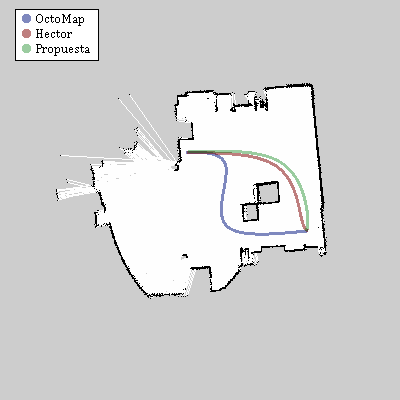
\includegraphics[width=0.5\textwidth]{figures/05experimentacion/r01.png}
    \caption{ Comparación de las trayectorias realizadas por los algoritmos en el ambiente 2} 
    \label{fig:tray_02}
    Fuente: Fabricación propia
\end{figure}

\newpage
\subsubsection{RESULTADOS EN EL AMBIENTE NÚMERO 3}

Los resultados producidos por el mapeo tridimensional y bidimensional del algoritmo propuesto durante la experimentación en el ambiente 3 se pueden apreciar en la Figura \ref{fig:ambiente_3} en donde al igual que en los ambientes anteriores, el mapeo se inició en la posición inicial, de esta manera dicha posición queda identificada en las coordenadas (0,0). Por otro lado, al interior del mapa generado se pueden apreciar el obstáculo 1, obstáculo 2 y el obstáculo 3.


\begin{figure}[H]
    \centering
    \begin{subfigure}[b]{0.30\textwidth}
    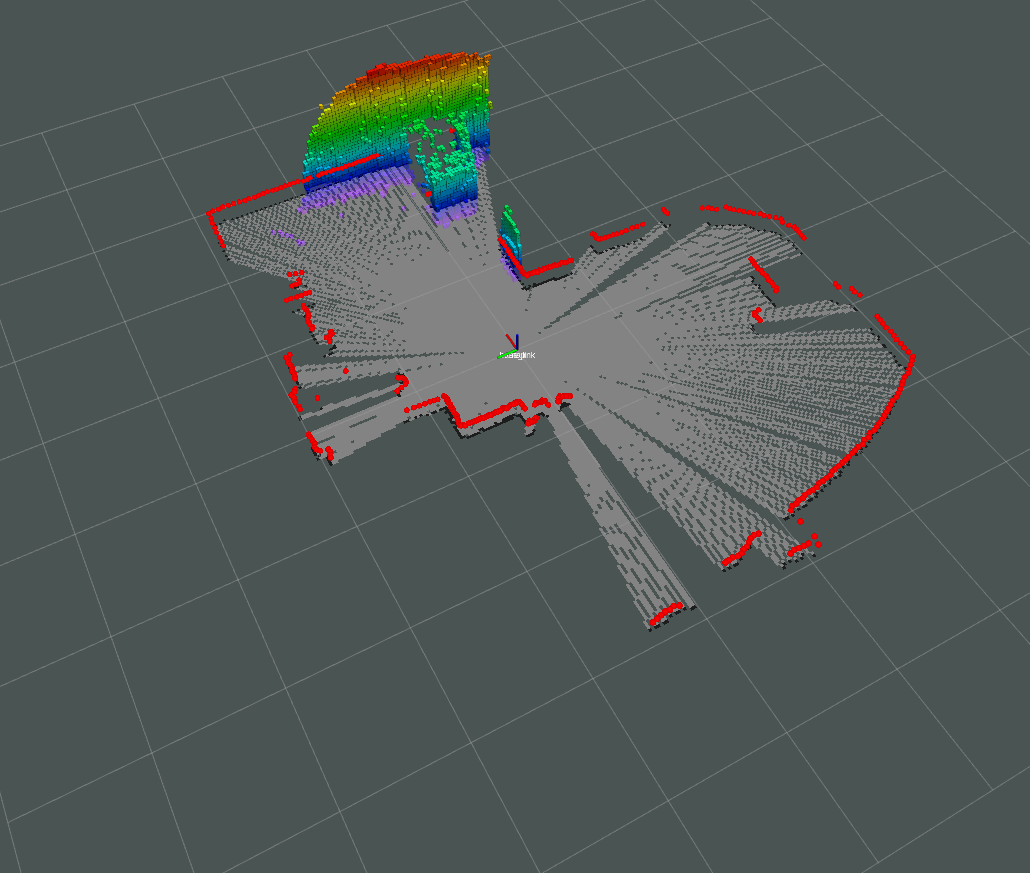
\includegraphics[width=\textwidth, height=\textwidth]{figures/05experimentacion/ambiente_3/r02_01.png}
    \caption{Inicio del mapeo}
    \label{fig:ambiente_3_1}
    \end{subfigure}
    \begin{subfigure}[b]{0.30\textwidth}
    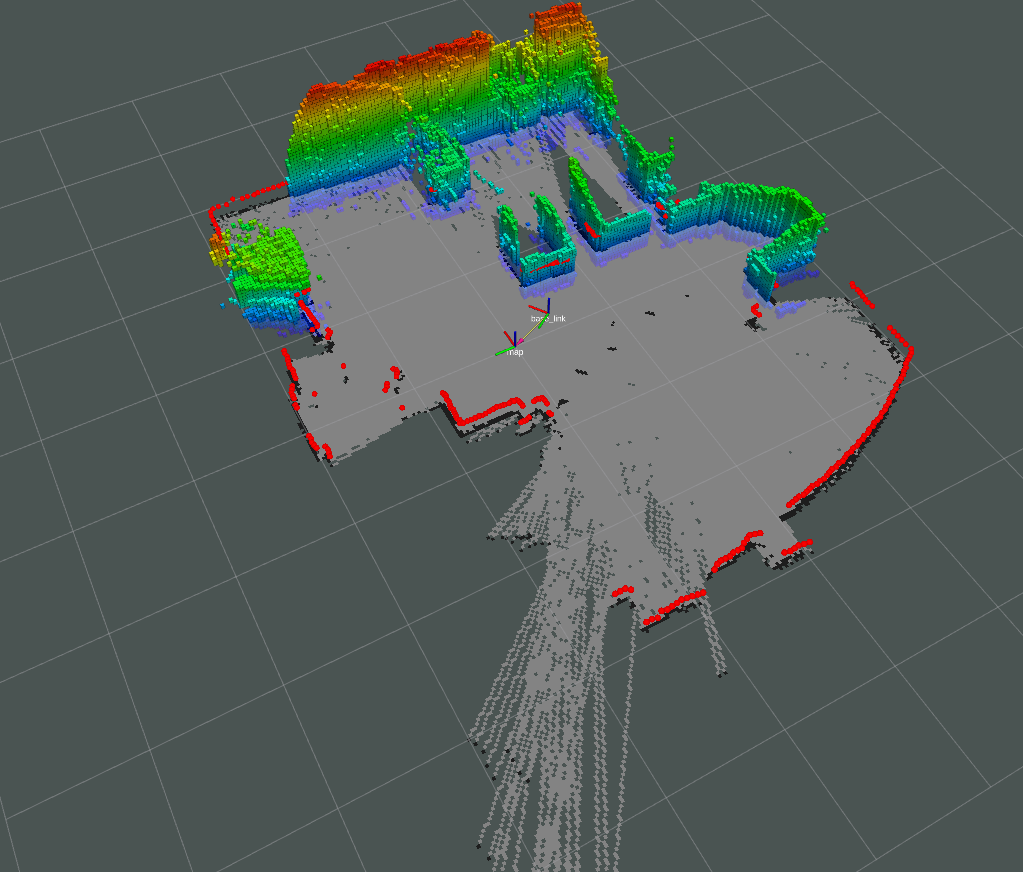
\includegraphics[width=\textwidth, height=\textwidth]{figures/05experimentacion/ambiente_3/r02_02.png}
    \caption{En proceso del mapeo}
    \label{fig:ambiente_3_2}
    \end{subfigure}
    \begin{subfigure}[b]{0.30\textwidth}
    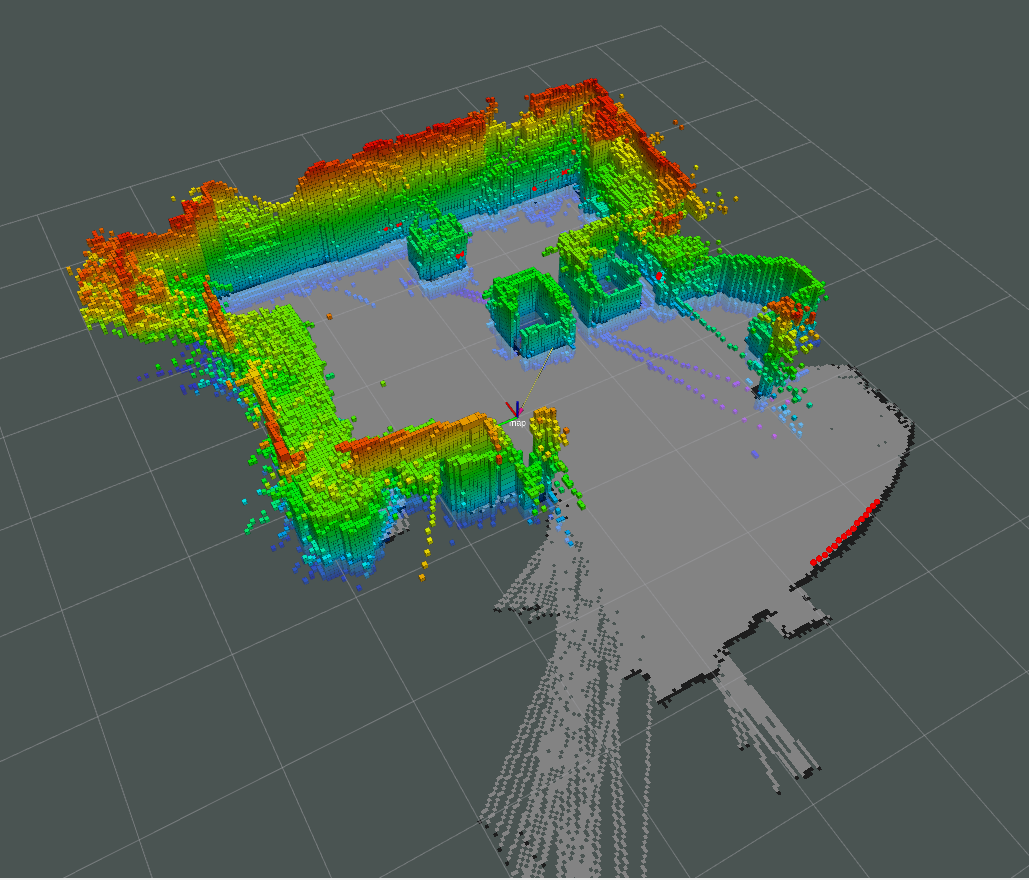
\includegraphics[width=\textwidth, height=\textwidth]{figures/05experimentacion/ambiente_3/r02_03.png}
    \caption{Ambiente mapeado}
    \label{fig:ambiente_3_3}
    \end{subfigure}
    \caption{Proceso de mapeo del ambiente 3}
    Fuente: Fabricación propia
    \label{fig:ambiente_3}
\end{figure} 

En la Tabla \ref{tab:resultados_ambiente_3} se detallan los resultados de las métricas evaluadas a cada algoritmo durante el reconocimiento y navegación por el ambiente 3. Al igual que en los experimentos anteriores, se observa como los algoritmos tridimensionales les toma más tiempo generar el mapa en comparación al algoritmo bidimensional. También se puede observar nuevamente un comportamiento favorable del algoritmo propuesto en comparación con el algoritmo OctoMap en las tareas asociadas al mapeo y en comparación al algoritmo Hector en las tareas asociadas a la navegación y localización, lo que marca una tendencia del comportamiento del algoritmo propuesto.

\begin{table}[H]
\centering
\begin{tabular}{@{}lccc@{}}
\toprule
\multicolumn{1}{|c|}{\textbf{Métrica}} &
  \multicolumn{1}{c|}{\textbf{OctoMap Library}} &
  \multicolumn{1}{c|}{\textbf{Hector Mapping}} &
  \multicolumn{1}{c|}{\textbf{Algoritmo Propuesto}} \\ \midrule
\multicolumn{1}{|l|}{\textbf{Tiempo en generar el mapa}}    & \multicolumn{1}{c|}{23,795} & \multicolumn{1}{c|}{8,962} & \multicolumn{1}{c|}{16,451} \\ \midrule
\multicolumn{1}{|l|}{\textbf{Precisión del mapa generado}}  & \multicolumn{1}{c|}{98,12\%} & \multicolumn{1}{c|}{95,246\%} & \multicolumn{1}{c|}{92,748\%} \\ \midrule
\multicolumn{1}{|l|}{\textbf{Ruta planificada}}             & \multicolumn{1}{c|}{7,278} & \multicolumn{1}{c|}{4,789} & \multicolumn{1}{c|}{4,957} \\ \midrule
\multicolumn{1}{|l|}{\textbf{Precisión de la ruta}}         & \multicolumn{1}{c|}{87,44\%} & \multicolumn{1}{c|}{91,25\%} & \multicolumn{1}{c|}{93,14\%} \\ \midrule
\multicolumn{1}{|l|}{\textbf{Tiempo en completar la ruta}}  & \multicolumn{1}{c|}{19,992} & \multicolumn{1}{c|}{9,347} & \multicolumn{1}{c|}{9,782} \\ \midrule
\multicolumn{1}{|l|}{\textbf{Tiempo de localización}}       & \multicolumn{1}{c|}{3,745} & \multicolumn{1}{c|}{1,174} & \multicolumn{1}{c|}{1,259} \\ \midrule
\multicolumn{1}{|l|}{\textbf{Precisión de la localización}} & \multicolumn{1}{c|}{81,75\%} & \multicolumn{1}{c|}{94,63\%} & \multicolumn{1}{c|}{97,78\%} \\ \midrule
\multicolumn{1}{|l|}{\textbf{Adaptación}}                   & \multicolumn{1}{c|}{True} & \multicolumn{1}{c|}{True} & \multicolumn{1}{c|}{True} \\ \midrule
\multicolumn{1}{|l|}{\textbf{Consumo de memoria}}           & \multicolumn{1}{c|}{1.949} & \multicolumn{1}{c|}{1.302} & \multicolumn{1}{c|}{2.578} \\ \midrule
\multicolumn{1}{|l|}{\textbf{Tamaño del archivo}}           & \multicolumn{1}{c|}{0,901} & \multicolumn{1}{c|}{0,027} & \multicolumn{1}{c|}{0,947} \\ \bottomrule
\end{tabular}
\caption{Resultados en Ambiente 3}
\label{tab:resultados_ambiente_3}
\end{table}

Por otro lado, en la Figura \ref{fig:tray_03} se identifican las trayectorias realizadas por los algoritmos en el experimento. A partir del aumento de obstáculos y dificultades a la hora de navegar en el ambiente, el comportamiento de los algoritmo se va marcando, es decir, el algoritmo OctoMap muestra una ruta ineficiente en comparación a los algoritmos Hector y al algoritmo propuesto, esto se debe a la construcción tridimensional que realiza el algoritmo y las imperfecciones propias de dicho algoritmo (dado que no está pensado en utilizarse con una cámara de profundidad), por otro lado la tendencia de similitud entre las trayectorias del algoritmo Hector y el algoritmo propuesto se sigue manteniendo.

\begin{figure}[h]
    \centering
    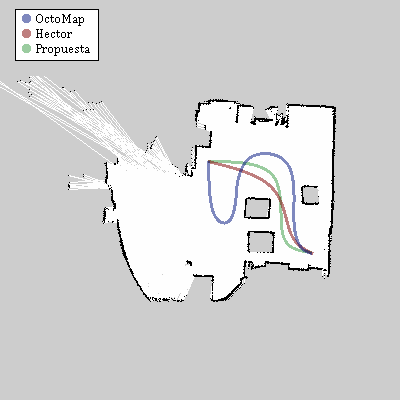
\includegraphics[width=0.5\textwidth]{figures/05experimentacion/r02.png}
    \caption{ Comparación de las trayectorias realizadas por los algoritmos en el ambiente 3} 
    \label{fig:tray_03}
    Fuente: Fabricación propia
\end{figure}

\newpage
\subsubsection{RESULTADOS EN EL AMBIENTE NÚMERO 4}

Durante la experimentación del ambiente 4 el robot se debió enfrentar además de los obstáculos a sub-puntos en la ruta, para ello se debió realizar el mapeo tridimensional y bidimensional al igual que en los ambientes anteriores, este proceso se puede observar en la Figura \ref{fig:ambiente_4}. También al igual en en los experimentos anteriores, el mapeo se inició en la posición inicial por lo que de esta manera dicha posición queda identificada en las coordenadas (0,0) dentro del mapa.


\begin{figure}[H]
    \centering
    \begin{subfigure}[b]{0.30\textwidth}
    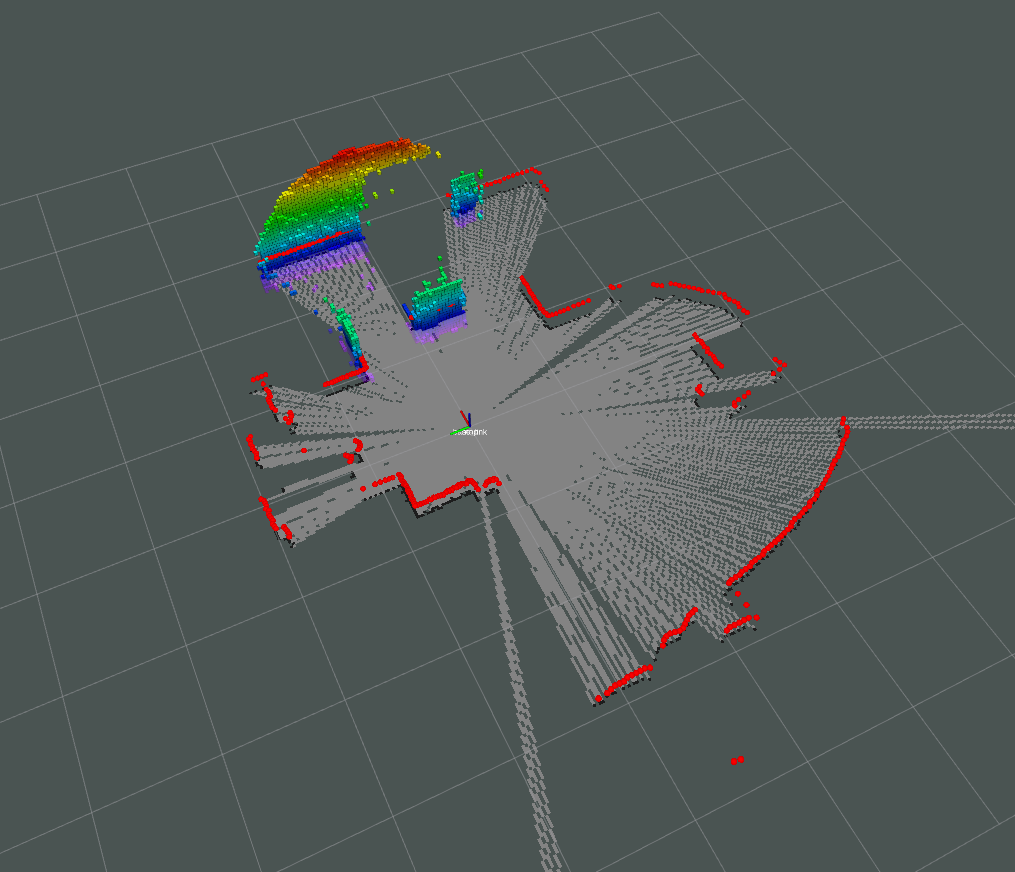
\includegraphics[width=\textwidth, height=\textwidth]{figures/05experimentacion/ambiente_4/r03_01.png}
    \caption{Inicio del mapeo}
    \label{fig:ambiente_4_1}
    \end{subfigure}
    \begin{subfigure}[b]{0.30\textwidth}
    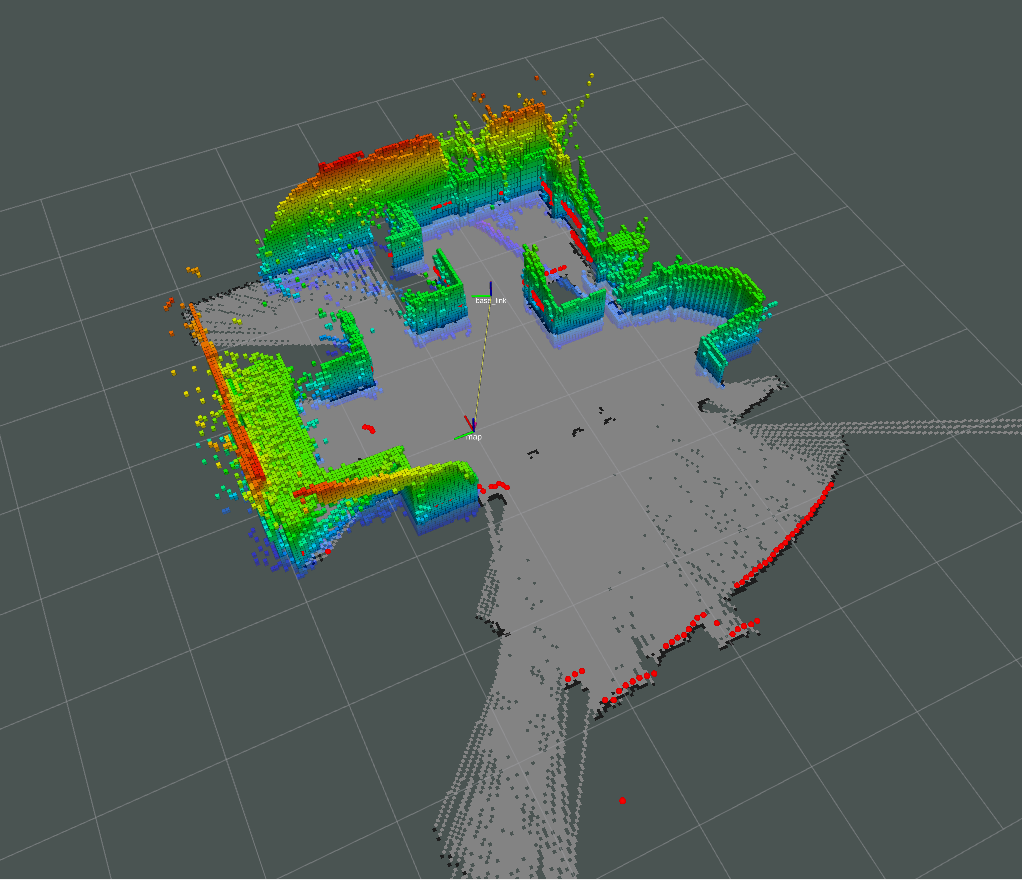
\includegraphics[width=\textwidth, height=\textwidth]{figures/05experimentacion/ambiente_4/r03_02.png}
    \caption{En proceso del mapeo}
    \label{fig:ambiente_4_2}
    \end{subfigure}
    \begin{subfigure}[b]{0.30\textwidth}
    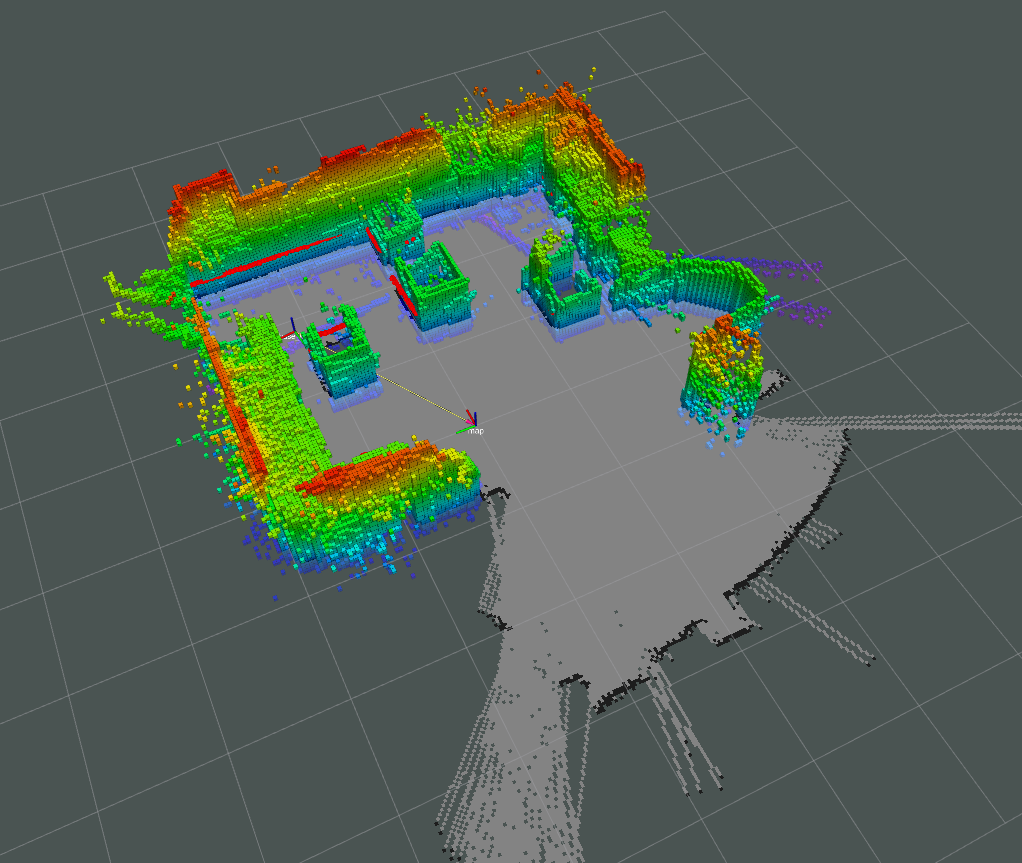
\includegraphics[width=\textwidth, height=\textwidth]{figures/05experimentacion/ambiente_4/r03_03.png}
    \caption{Ambiente mapeado}
    \label{fig:ambiente_4_3}
    \end{subfigure}
    \caption{Proceso de mapeo del ambiente 4}
    Fuente: Fabricación propia
    \label{fig:ambiente_4}
\end{figure} 

Los resultados obtenidos por cada algoritmo se pueden observar en la Tabla \ref{tab:resultados_ambiente_4}, aquí se detallan los resultados obtenidos durante la experimentación en el ambiente 4. La tendencia obtenida durante el desarrollo de los experimentos anteriores se sigue marcando, es decir, a los algoritmos tridimensionales les tarda más tiempo construir el mapa en comparación con el algoritmo bidimensional.

Se observa como cambia drásticamente la precisión del algoritmo OctoMap a la hora de ubicarse, lo mismo ocurre con la precisión de la ruta planificada. Esta diferencia de resultados en comparación con los experimentos desarrollados anteriormente, se da ya que en este ambiente se agrega un sub-punto en la ruta, lo que dificulta la tarea de navegar.


\begin{table}[H]
\centering
\begin{tabular}{@{}lccc@{}}
\toprule
\multicolumn{1}{|c|}{\textbf{Métrica}} &
  \multicolumn{1}{c|}{\textbf{OctoMap Library}} &
  \multicolumn{1}{c|}{\textbf{Hector Mapping}} &
  \multicolumn{1}{c|}{\textbf{Algoritmo Propuesto}} \\ \midrule
\multicolumn{1}{|l|}{\textbf{Tiempo en generar el mapa}}    & \multicolumn{1}{c|}{29,041} & \multicolumn{1}{c|}{11,237} & \multicolumn{1}{c|}{21,998} \\ \midrule
\multicolumn{1}{|l|}{\textbf{Precisión del mapa generado}}  & \multicolumn{1}{c|}{96,08\%} & \multicolumn{1}{c|}{92,01\%} & \multicolumn{1}{c|}{95,41\%} \\ \midrule
\multicolumn{1}{|l|}{\textbf{Ruta planificada}}             & \multicolumn{1}{c|}{16,476} & \multicolumn{1}{c|}{8,554} & \multicolumn{1}{c|}{9,678} \\ \midrule
\multicolumn{1}{|l|}{\textbf{Precisión de la ruta}}         & \multicolumn{1}{c|}{76,88\%} & \multicolumn{1}{c|}{88,416\%} & \multicolumn{1}{c|}{95,24\%} \\ \midrule
\multicolumn{1}{|l|}{\textbf{Tiempo en completar la ruta}}  & \multicolumn{1}{c|}{39,045} & \multicolumn{1}{c|}{17,875} & \multicolumn{1}{c|}{22,045} \\ \midrule
\multicolumn{1}{|l|}{\textbf{Tiempo de localización}}       & \multicolumn{1}{c|}{3,947} & \multicolumn{1}{c|}{2,014} & \multicolumn{1}{c|}{1,114} \\ \midrule
\multicolumn{1}{|l|}{\textbf{Precisión de la localización}} & \multicolumn{1}{c|}{71,01\%} & \multicolumn{1}{c|}{95,47\%} & \multicolumn{1}{c|}{96,27\%} \\ \midrule
\multicolumn{1}{|l|}{\textbf{Adaptación}}                   & \multicolumn{1}{c|}{True} & \multicolumn{1}{c|}{True} & \multicolumn{1}{c|}{True} \\ \midrule
\multicolumn{1}{|l|}{\textbf{Consumo de memoria}}           & \multicolumn{1}{c|}{2.009} & \multicolumn{1}{c|}{1.405} & \multicolumn{1}{c|}{2.997} \\ \midrule
\multicolumn{1}{|l|}{\textbf{Tamaño del archivo}}           & \multicolumn{1}{c|}{0,870} & \multicolumn{1}{c|}{0,031} & \multicolumn{1}{c|}{0,884} \\ \bottomrule
\end{tabular}
\caption{Resultados en Ambiente 4}
\label{tab:resultados_ambiente_4}
\end{table}

Con respecto a las trayectorias realizadas por los 3 algoritmos, estas se pueden observar en la Figura \ref{fig:tray_04}. Se observa la tendencia que hace alusión al comportamiento a la hora de planificar una ruta entre el algoritmo Hector y el algoritmo de la propuesta.

Ambos algoritmos determinan la ruta más eficiente a la hora de planificar la ruta lo que conlleva a un comportamiento similar, sin embargo, el algoritmo OctoMap tiene un comportamiento totalmente diferente a la hora de generar la ruta lo que genera vueltas innecesarias durante la experimentación.

\begin{figure}[h]
    \centering
    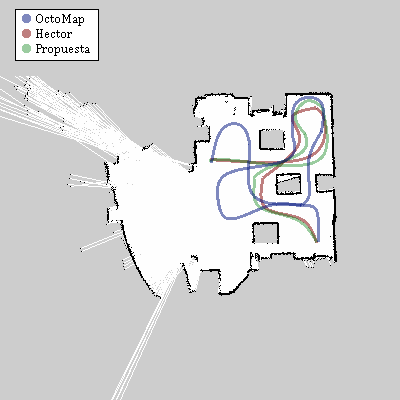
\includegraphics[width=0.5\textwidth]{figures/05experimentacion/r03.png}
    \caption{ Comparación de las trayectorias realizadas por los algoritmos en el ambiente 4} 
    \label{fig:tray_04}
    Fuente: Fabricación propia
\end{figure}

\newpage
\subsubsection{RESULTADOS EN EL AMBIENTE NÚMERO 5}

\begin{figure}[H]
    \centering
    \begin{subfigure}[b]{0.30\textwidth}
    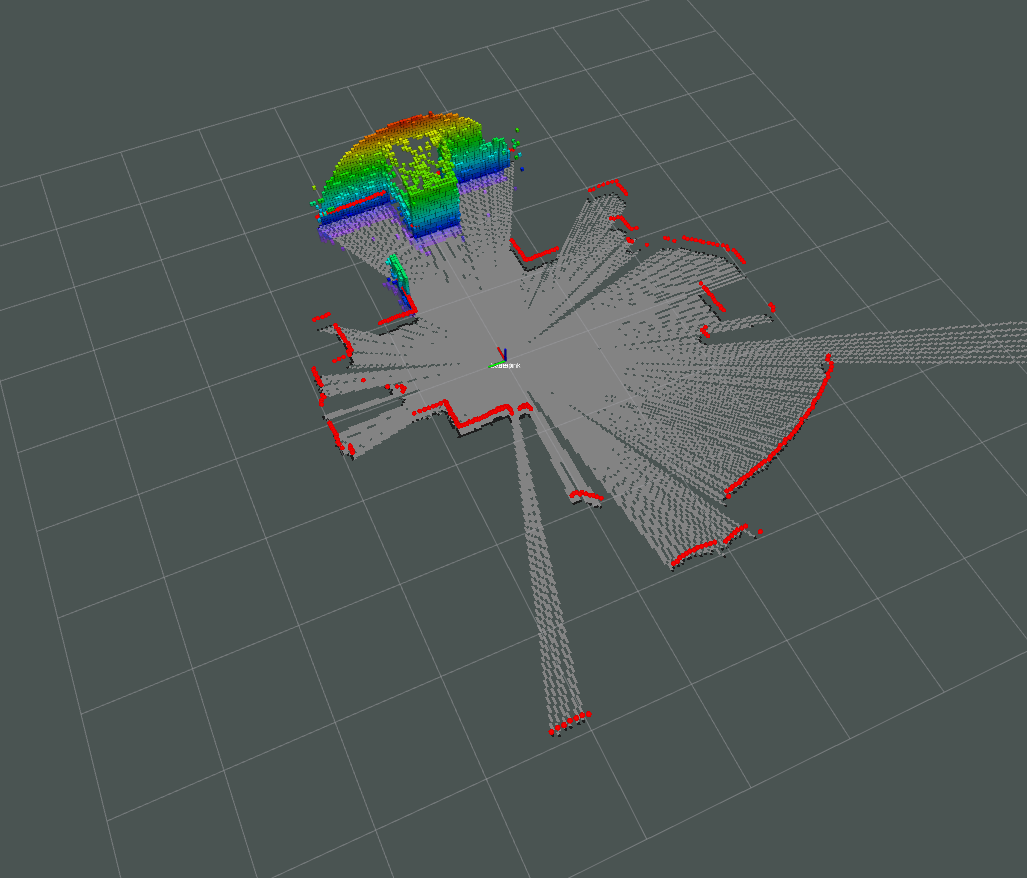
\includegraphics[width=\textwidth, height=\textwidth]{figures/05experimentacion/ambiente_5/r04_01.png}
    \caption{Inicio del mapeo}
    \label{fig:ambiente_5_1}
    \end{subfigure}
    \begin{subfigure}[b]{0.30\textwidth}
    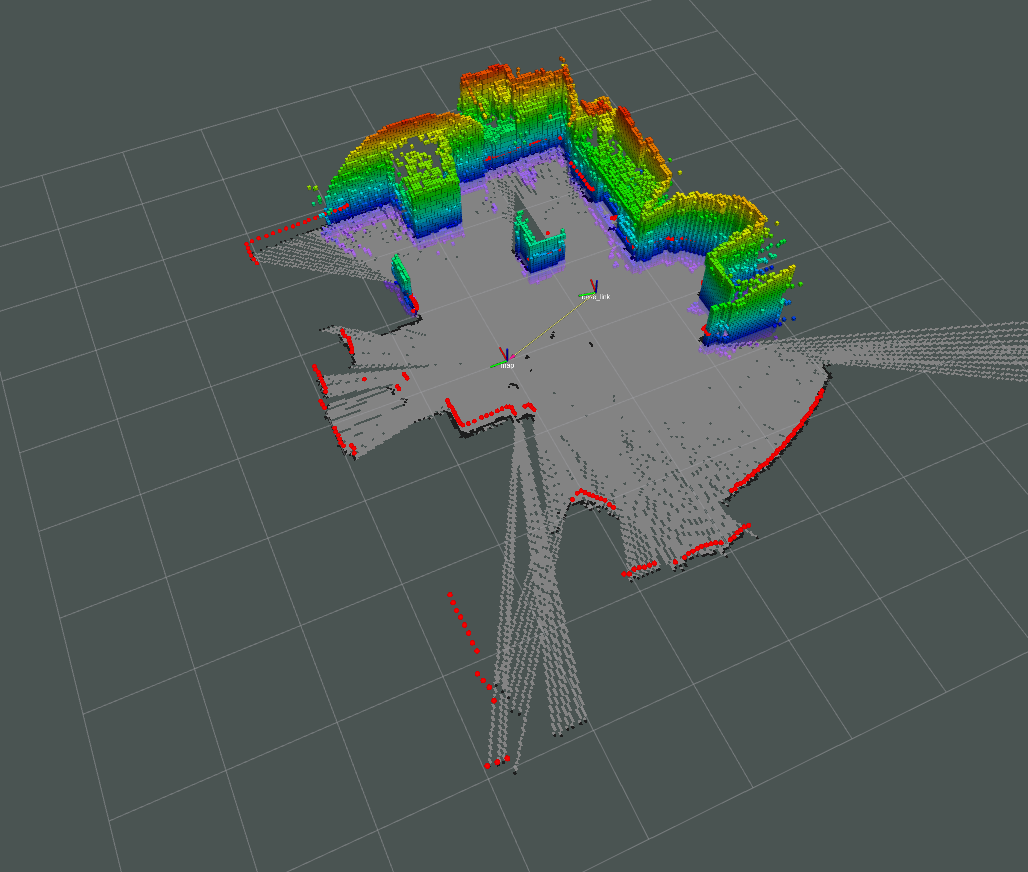
\includegraphics[width=\textwidth, height=\textwidth]{figures/05experimentacion/ambiente_5/r04_02.png}
    \caption{En proceso del mapeo}
    \label{fig:ambiente_5_2}
    \end{subfigure}
    \begin{subfigure}[b]{0.30\textwidth}
    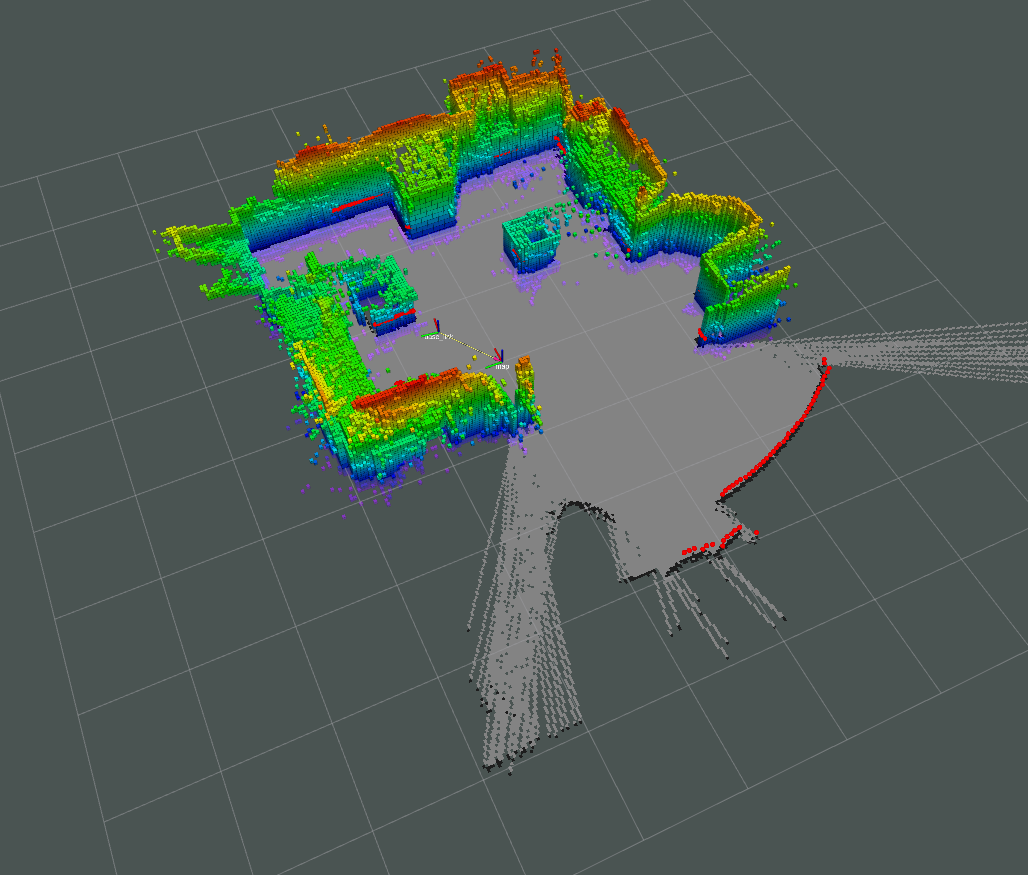
\includegraphics[width=\textwidth, height=\textwidth]{figures/05experimentacion/ambiente_5/r04_03.png}
    \caption{Ambiente mapeado}
    \label{fig:ambiente_5_3}
    \end{subfigure}
    \caption{Proceso de mapeo del ambiente 5}
    Fuente: Fabricación propia
    \label{fig:ambiente_5}
\end{figure} 

En el último ambiente testeado, además de que el robot debía ir desde la posición inicial hasta la posición final posando por un sub-punto intermedio con la salvación de que existen zonas prohibidas las cuales al momento de pasar por encime se agrega una penalización. Para realizar esta tarea el algoritmo debió mapear tridimensional y bidimensionalmente el entorno, este proceso se puede analizar en la Figura \ref{fig:ambiente_5}.

Al igual que en los experimentos anteriores,  el mapeo se inició en la posición inicial por lo que de esta manera dicha posición queda identificada en las coordenadas (0,0) dentro del mapa y también se pueden observar los 3 obstáculos como también las zonas prohibidas detectadas por el algoritmo.

Los resultados obtenidos en este último ambiente se detallan en la Tabla \ref{tab:resultados_ambiente_5}, se puede apreciar como la tendencia marcada en los ambientes anteriores se sigue manteniendo. Cabe destacar que dado que tanto el algoritmo de OctoMap como el algoritmo Hector no presentan forma alguna de distinguir áreas prohibidas presentan una menor precisión del mapa y también no son capaces de adaptarse a los cambios presentes en este tipo de situaciones. 

Por otra parte, también se nota como la precisión del algoritmo propuesto, es decir, la precisión en el mapa generado, la precisión en la ruta y la precisión en la localización, se mantienen estable. Se pueden destacar también que el algoritmo OctoMap presenta 3 penalizaciones debido a que entro en 3 ocasiones a las zonas prohibidas, mientras que el algoritmo Hector presenta 2 penalizaciones por las mismas razones, dichas penalizaciones se ven reflejadas en un porcentaje de aumento según la cantidad de penalizaciones obtenidas en el valor de la ruta planificada y en el valor del tiempo en completar la ruta, en estas métricas el valor original aparece en paréntesis mientras que por su parte, el valor con la penalización incluida se presenta sin paréntesis.

\begin{table}[H]
\centering
\begin{tabular}{@{}lccc@{}}
\toprule
\multicolumn{1}{|c|}{\textbf{Métrica}} &
  \multicolumn{1}{c|}{\textbf{OctoMap Library}} &
  \multicolumn{1}{c|}{\textbf{Hector Mapping}} &
  \multicolumn{1}{c|}{\textbf{Algoritmo Propuesto}} \\ \midrule
\multicolumn{1}{|l|}{\textbf{Tiempo en generar el mapa}}    & \multicolumn{1}{c|}{33,646} & \multicolumn{1}{c|}{12,198} & \multicolumn{1}{c|}{23,702} \\ \midrule
\multicolumn{1}{|l|}{\textbf{Precisión del mapa generado}}  & \multicolumn{1}{c|}{72,05\%} & \multicolumn{1}{c|}{75,41\%} & \multicolumn{1}{c|}{95,04\%} \\ \midrule
\multicolumn{1}{|l|}{\textbf{Ruta planificada}}             & \multicolumn{1}{c|}{22,250 (17,115)} & \multicolumn{1}{c|}{ 16,405 (13,671) } & \multicolumn{1}{c|}{9,678} \\ \midrule
\multicolumn{1}{|l|}{\textbf{Precisión de la ruta}}         & \multicolumn{1}{c|}{77,26\%} & \multicolumn{1}{c|}{94,06\%} & \multicolumn{1}{c|}{95,05\%} \\ \midrule
\multicolumn{1}{|l|}{\textbf{Tiempo en completar la ruta}}  & \multicolumn{1}{c|}{45,603 (35,079)} & \multicolumn{1}{c|}{22,494 (18,745)} & \multicolumn{1}{c|}{23,048} \\ \midrule
\multicolumn{1}{|l|}{\textbf{Tiempo de localización}}       & \multicolumn{1}{c|}{4,034} & \multicolumn{1}{c|}{2,045} & \multicolumn{1}{c|}{1,772} \\ \midrule
\multicolumn{1}{|l|}{\textbf{Precisión de la localización}} & \multicolumn{1}{c|}{73,01\%} & \multicolumn{1}{c|}{94,01\%} & \multicolumn{1}{c|}{98,71\%} \\ \midrule
\multicolumn{1}{|l|}{\textbf{Adaptación}}                   & \multicolumn{1}{c|}{False} & \multicolumn{1}{c|}{False} & \multicolumn{1}{c|}{True} \\ \midrule
\multicolumn{1}{|l|}{\textbf{Consumo de memoria}}           & \multicolumn{1}{c|}{2.117} & \multicolumn{1}{c|}{1.301} & \multicolumn{1}{c|}{3.778} \\ \midrule
\multicolumn{1}{|l|}{\textbf{Tamaño del archivo}}           & \multicolumn{1}{c|}{0,927} & \multicolumn{1}{c|}{0,037} & \multicolumn{1}{c|}{1,023} \\ \bottomrule
\end{tabular}
\caption{Resultados en Ambiente 5}
\label{tab:resultados_ambiente_5}
\end{table}

Las trayectorias planificadas por los algoritmos en este último ambiente así como también las zonas prohibidas se pueden apreciar en la Figura \ref{fig:tray_05}. En este caso se puede apreciar que cada algoritmo realiza una trayectoria distinta, sin embargo, la tendencia de que las rutas planificadas por el algoritmo OctoMap son ineficientes se mantiene, también se puede observar que las trayectorias realizadas tanto por el algoritmo Hector como las realizadas por el algoritmo OctoMap no toman en cuenta las zonas prohibidas.

También se observa como el consumo de memoria del algoritmo propuesto aumenta si el entorno es más complejo de mapear, navegar o si presenta zonas prohibidas. Por otro lado, al igual que en el ambiente 4, el algoritmo OctoMap tiene un comportamiento peor a la hora de generar las rutas dando resultados totalmente ineficientes y en ocasiones, contraproducentes.


\begin{figure}[h]
    \centering
    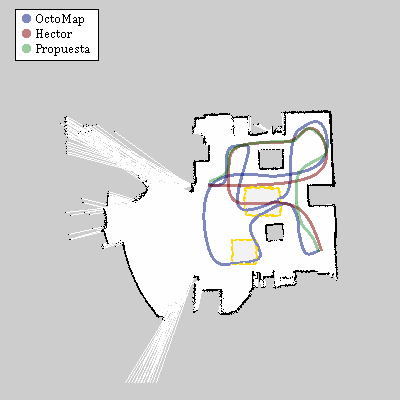
\includegraphics[width=0.4\textwidth]{figures/05experimentacion/r04.png}
    \caption{ Comparación de las trayectorias realizadas por los algoritmos en el ambiente 5} 
    \label{fig:tray_05}
    Fuente: Fabricación propia
\end{figure}

